%-----------------------------------------------------------------------------
%
%               Template for sigplanconf LaTeX Class
%
% Name:         sigplanconf-template.tex
%
% Purpose:      A template for sigplanconf.cls, which is a LaTeX 2e class
%               file for SIGPLAN conference proceedings.
%
% Guide:        Refer to "Author's Guide to the ACM SIGPLAN Class,"
%               sigplanconf-guide.pdf
%
% Author:       Paul C. Anagnostopoulos
%               Windfall Software
%               978 371-2316
%               paul@windfall.com
%
% Created:      15 February 2005
%
%-----------------------------------------------------------------------------


\documentclass{sigplanconf}

% The following \documentclass options may be useful:

% preprint      Remove this option only once the paper is in final form.
% 10pt          To set in 10-point type instead of 9-point.
% 11pt          To set in 11-point type instead of 9-point.
% authoryear    To obtain author/year citation style instead of numeric.

\usepackage{amsmath}
\usepackage{amsthm}
\usepackage{bm}
\usepackage{tikz}
\usetikzlibrary{decorations.markings}
\usetikzlibrary{positioning}
\tikzstyle{vertex}=[circle, draw, inner sep=0pt, minimum size=6pt]

\begin{document}

\special{papersize=8.5in,11in}
\setlength{\pdfpageheight}{\paperheight}
\setlength{\pdfpagewidth}{\paperwidth}

\conferenceinfo{CONF 'yy}{Month d--d, 20yy, City, ST, Country}
\copyrightyear{20yy}
\copyrightdata{978-1-nnnn-nnnn-n/yy/mm}
\doi{nnnnnnn.nnnnnnn}

% Uncomment one of the following two, if you are not going for the
% traditional copyright transfer agreement.

%\exclusivelicense                % ACM gets exclusive license to publish,
                                  % you retain copyright

%\permissiontopublish             % ACM gets nonexclusive license to publish
                                  % (paid open-access papers,
                                  % short abstracts)

\titlebanner{banner above paper title}        % These are ignored unless
\preprintfooter{short description of paper}   % 'preprint' option specified.

\title{Elizabeth Scott Explained}
\subtitle{Parsing from Earley Recognisers}

\authorinfo{Zoe Wheeler}
           {University of Texas at Austin}
           {zoe.donnellon.wheeler@gmail.com}
\authorinfo{Walter Xia}
           {University of Texas at Austin}
           {swilery@utexas.edu}

\maketitle

\begin{abstract}
Earley's Algorithm is able to recognize general context-free grammars in $O(n^3)$, where $n$ is the size of the string to be recognized. However, there are times in which we want more than just a yes or no answer. There are times in which we want an actual parse tree, and for ambiguous grammars, there are times in which we want all possible parse trees. Fortunately, there is a paper by Dr. Elizabeth Scott, \cite{scott}, that presents a technique to produce a data structure known as a Shared Packed Parse Forest (SPPF), able to represent even an infinite number of parse trees. Unfortunately this paper is poorly written, making it very difficult to understand. Our paper is a re-explanation of Scott's techniques. It is agreed by many that Earley's Algorithm is also difficult to understand. Fortunately, there exists a data structure due to Dr. Gianfranco Bilardi and Dr. Keshav Pingali, \cite{bilardi-pingali}, known as Grammar Flow Graphs (GFGs) that significantly ease the understanding of the algorithm by reformulating parsing problems as path problems in a graph. Our technique will use GFGs.
\end{abstract}

\category{F.7.2}{Semantics and Reasoning}{Program Reasoning--Parsing}

% general terms are not compulsory anymore,
% you may leave them out
\terms
Context-Free Languages, Cubic Generalized Parsing, Earley Parsing 

\keywords
Earley Sets, Grammar Flow Graphs, Non-Deterministic Finite Automaton, Shared Packed Parse Forest

\section{Introduction}
It is important here for us to distinguish between recognisers and parsers for a grammar. Recognizers determine whether or not a string is part of a language defined by a grammar whereas parsers construct parse trees that reveal \textit{how} a string satisfies the syntax dictated by a grammar. For about the past five decades, there already exist general recognizers like Cocke-Younger-Kasami (CYK) and Earley's Algorithms that run cubic relative to the size of the string to be recognized. Alternatively, Generalized LR (GLR) is an algorithm that produces parsers but has the very undesirable property that it is unbounded. Dr. Elizabeth Scott extended the Earley Recogniser into a parser that is able run in cubic space and time, \cite{scott}. The challenge was to successfully apply the parser to ambiguous grammars that produces multiple, perhaps infinite, parse trees for a string in the grammar. Note that simply disallowing ambiguous grammars is not a solution since there exists grammars that are intrinsically ambiguous. The solution she used was a representation known as a Shared Packed Parse Forest (SPPF), which is in essence a Directed Acyclic Graph (DAG).

Earley's Algorithm is a highly complex algorithm. To dramatically simplify its understanding, we view it from the perspective of Grammar Flow Graphs (GFGs) that restructure parsing as finding certain paths within the graph, \cite{bilardi-pingali}. For those of you familiar with automata theory, GFGs play the same role for context-free grammars as finite-state automota play for regular grammars. The rest of the paper is organized as follows:
\begin{itemize}
\item Section 2 will introduce GFGs
\item Section 3 will introduce Earley's Algorithm using GFGs
\item Section 4 will introduce SPPFs
\item Section 5 will introduce Dr. Scott's Algorithm for producing SPPFs
\item Section 6 will discuss our implementation
\item Section 7 will discuss our results
\item Section 8 will conclude
\end{itemize}

\section{Grammar Flow Graphs}
Let us begin with the standard definition of a context-free grammar.

\textit{Definition:} A \textit{context-free grammar}, \textit{CFG}, is a tuple $(N, T, P, S)$, where, \cite{bilardi-pingali}:
\begin{itemize}
\item[$\triangleright$] $N$ is a finite set of elements called \textit{nonterminals}, 
\item[$\triangleright$] $T$ is a finite set of elements called \textit{terminals}, 
\item[$\triangleright$] $P\subseteq{N\times{(N\cup{T}}})^*$ is the set of \textit{productions} that map nonterminals to a sequence of nonterminals or terminals, and 
\item[$\triangleright$] $S\in{N}$ is the unique \textit{start symbol} that appears once on the left-hand side of a single production.
\end{itemize}

An example of a grammar is the following, where $|$ signifies or:
\begin{align*}
S&\longrightarrow{N \: t \: | \: t \: N} \\
N&\longrightarrow{t \: t}
\end{align*}

Now we are in a position to introduce the GFG.

\textit{Definition:} Let $CFG = (N, T, P, S)$ be a context-free grammar and let $\epsilon$ denote the empty string. The \textit{grammar flow graph (GFG)} of $CFG$, $GFG(CFG) = (V(CGF), G(CFG))$, is the smalled directed graph that has the following properties, \cite{bilardi-pingali}:
\begin{itemize}
\item[$\triangleright$] For each nonterminal $M\in{N}$, there exist $(\bullet{M})$,$(M\bullet){\in{V(CFG)}}$ called \textit{start nodes} and \textit{end nodes} respectively,
\item[$\triangleright$] For each production $(M\longrightarrow{\epsilon})\in{P}$, there exists $(M\longrightarrow{\bullet})\in{V(CFG)}$ and $(\bullet{M}, M\longrightarrow{\bullet}),(M\longrightarrow{\bullet}, M\bullet)\in{E(CFG)}$,
\item[$\triangleright$] For each production $(M\longrightarrow{q_1q_2\dots{q_r}})$ where $q_i \neq \epsilon$:
\begin{itemize}
\item[$\diamond$] $(M\longrightarrow{\bullet{q_1q_2\dots{q_r}}}), (M\longrightarrow{q_1\bullet{q_2\dots{q_r}}}), \dots, (M\longrightarrow{q_1q_2...q_r\bullet})\in{V(CFG)}$, where the first node is called an \textit{entry node} and the last node is called an \textit{exit node},
\item[$\diamond$] $(\bullet{M}, M\longrightarrow{\bullet{q_1q_2\dots{q_r}}}), (M\longrightarrow{q_1q_2\dots{q_r\bullet}}, M\bullet)\in{E(CFG)}$ called \textit{entry edges} and \textit{exit edges} respectively,
\item[$\diamond$] For each $t\in{T}$, $(M\longrightarrow{\dots{\bullet{t\dots}}}, M\longrightarrow{\dots{t\bullet{\dots}}})\in{E(CFG)}$ called \textit{scan edges} labeled $t$, where $(M\longrightarrow{\dots{\bullet{t\dots}}})$ is called a \textit{scan node}, and
\item[$\diamond$] For each $K\in{N}$, $(M\longrightarrow{\dots{\bullet{K\dots}}}, \bullet{K})$, $(K\bullet, M\longrightarrow{\dots{K\bullet{\dots}}})$ called \textit{call edges} and \textit{return edges} respectively, where $(M\longrightarrow{\dots{\bullet{K\dots}}})$ is called a \textit{call node} that is matched with the \textit{return node} $(M\longrightarrow{\dots{K\bullet{\dots}}})$, and
\end{itemize}
\item[$\triangleright$] Edges not scan edges are labeled $\epsilon$.
\end{itemize}
\begin{figure}
\begin{center}
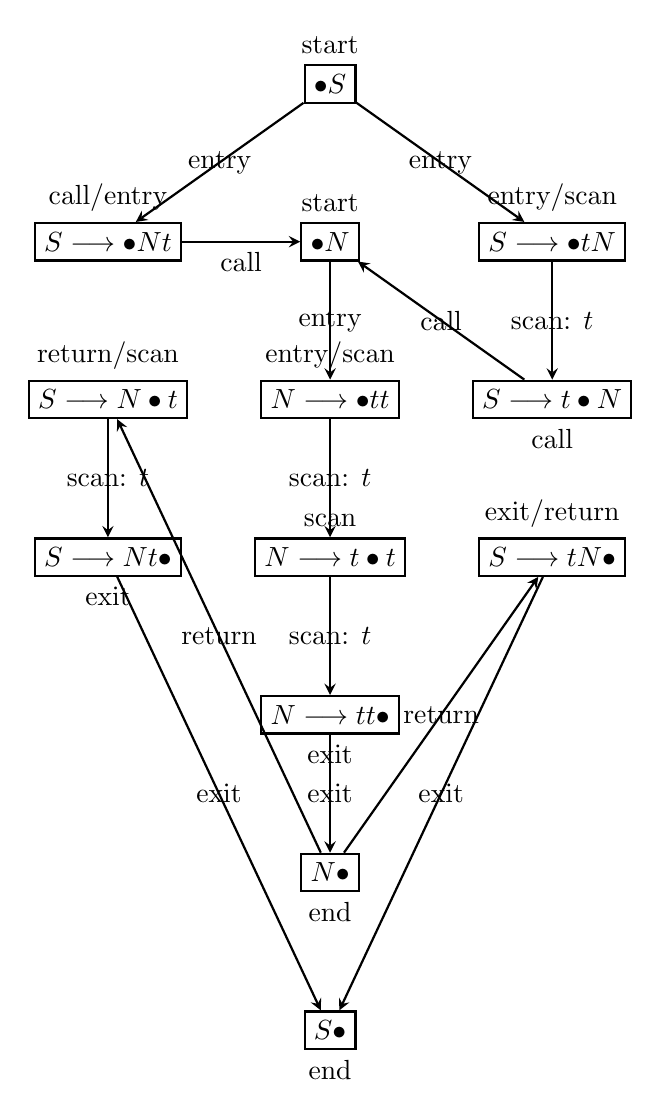
\begin{tikzpicture}[->,>=stealth,node distance = 1.5cm,thick]
\tikzstyle{v}=[rectangle,minimum size=1mm,draw,thick]
\node[v, label=start]	(dotS)  					   		{$\bullet{S}$};
\node[v, label=start] 	(dotN)  	[below = of dotS]		{$\bullet{N}$};
\node[v, label=entry/scan] 	(dottt)  	[below = of dotN]		{$N\longrightarrow{\bullet{tt}}$};
\node[v, label=scan] 	(tdott)  	[below = of dottt]		{$N\longrightarrow{t\bullet{t}}$};
\node[v, label={[below = 0.5cm]:exit}] 	(ttdot)  	[below = of tdott]		{$N\longrightarrow{tt\bullet}$};
\node[v, label={[below = 0.5cm]:end}] 	(Ndot)  	[below = of ttdot]		{$N\bullet$};
\node[v, label={[below = 0.5cm]:end}] 	(Sdot)  	[below = of Ndot]		{$S\bullet$};
\node[v, label=call/entry] 	(dotNt)		[left = of dotN]		{$S\longrightarrow{\bullet{Nt}}$};
\node[v, label=return/scan] 	(Ndott)  	[below = of dotNt]		{$S\longrightarrow{N\bullet{t}}$};
\node[v, label={[below = 0.5cm]:exit}] 	(Ntdot)  	[below = of Ndott]		{$S\longrightarrow{Nt\bullet}$};
\node[v, label=entry/scan] 	(dottN)  	[right = of dotN]		{$S\longrightarrow{\bullet{tN}}$};
\node[v, label={[below = 0.5cm]:call}] 	(tdotN)  	[below = of dottN]		{$S\longrightarrow{t\bullet{N}}$};
\node[v, label=exit/return] 	(tNdot)  	[below = of tdotN]		{$S\longrightarrow{tN\bullet}$};
\path(dotS)		edge	node			{entry}		(dotNt)
	 (dotS)		edge	node			{entry}		(dottN)
	 (dotNt)	edge	node[below]			{call}		(dotN)
	 (tdotN)	edge	node			{call}		(dotN)
	 (dotN)		edge	node			{entry}		(dottt)
	 (dottt)	edge	node		{scan: $t$}	(tdott)
	 (tdott)	edge	node		{scan: $t$}	(ttdot)
	 (ttdot)	edge	node			{exit}		(Ndot)
	 (Ndot)		edge	node			{return}		(Ndott)
	 (Ndot)		edge	node			{return}		(tNdot)
	 (Ndott)	edge	node		{scan: $t$}	(Ntdot)
	 (dottN)	edge	node		{scan: $t$}	(tdotN)
	 (Ntdot)	edge	node			{exit}		(Sdot)
	 (tNdot)	edge	node			{exit}		(Sdot);
\end{tikzpicture}
\caption{Example of a GFG for the preceding grammar.} \label{fig:M1}
\end{center}	
\end{figure}

Figure \ref{fig:M1} depicts the GFG associated with the preceding grammar. The following definition comes naturally.

\textit{Definition}: A path in a GFG \textit{generates} the word $w$ by concatenating the labels along its sequence of edges.

Those familiar with automata theory may recognize that a GFG resembles a non-deterministic finite-state automaton (NFA) which starts at $\bullet{S}$ and accepts at $S\bullet$. The idea is that each path from $\bullet{S}$ to $S\bullet$ generates a word recognized by the automaton. However, in general, this is not the case. To see this, consider the path $P = (\bullet{S}, S\longrightarrow{\bullet{tN}}, S\longrightarrow{t\bullet{N}}, \bullet{N}, N\longrightarrow{\bullet{tt}}, N\longrightarrow{t\bullet{t}}, N\longrightarrow{tt\bullet}, N\bullet, S\longrightarrow{N\bullet{t}}, S\longrightarrow{Nt\bullet}, S\bullet)$ in Figure \ref{fig:M1}. $P$ generates the word "tttt" which is not part of the original grammar. To maintain correctness, we must restrict the valid paths the automaton can take. In the case of $P$, the automaton must realize that after traversing the edge $(S\longrightarrow{t\bullet{N}}, \bullet{N})$ it must traverse $(N\bullet, S\longrightarrow{tN\bullet})$ instead of $(N\bullet, S\longrightarrow{N\bullet{t}})$. In general, the automaton can choose an arbitrary outgoing edge at a start node but at an end node, it must choose the return edge corresponding to the call edge it took. This behavior can be represented by a stack, by which when the automaton encounters a call node, it pushes the corresponding return node on the stack. Subsequently at an end node, the automaton pops the stack. In the case of $P$, $(S\longrightarrow{tN\bullet})$ gets pushed on the stack at $(S\longrightarrow{t\bullet{N}}$) and it gets popped at $N\bullet$. Dr. Bilardi and Pingali called this automaton a non-deterministic GFG automaton (NGA). We have the following definition.

\textit{Definition}: The valid paths a NGA could follow from $\bullet{S}$ to $S\bullet$ are called \textit{complete balanced paths (CBPs)}.

\textit{Theorem 1}: Let $CFG = (N, T, P, S)$ and let $w\in{T^*}$. $w$ is part of the language produced by $CFG$ iff a CBP of GFG(CFG) generates $w$.

\textit{Proof}: Please see \cite{bilardi-pingali}.

\begin{figure}
\begin{center}
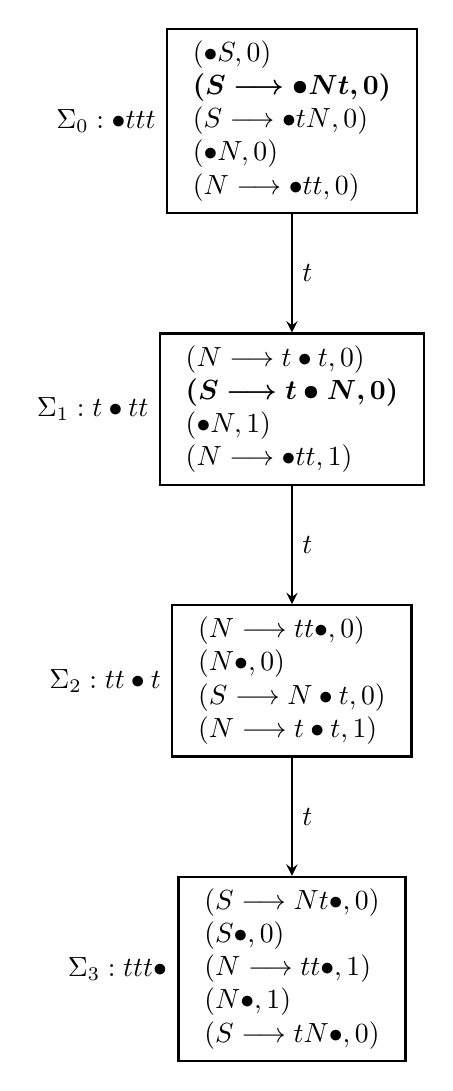
\begin{tikzpicture}[->,>=stealth,node distance = 1.5cm,thick]
\tikzstyle{v}=[rectangle,minimum size=1mm,draw,thick]
\node[v, label=left:$\Sigma_0:\bullet{ttt}$]	(S0)  					   		{\begin{tabular}{l}
  $(\bullet{S}, 0)$\\
  \bm{$(S\longrightarrow{\bullet{Nt}}, 0)$}\\
  $(S\longrightarrow{\bullet{tN}}, 0)$\\
  $(\bullet{N}, 0)$\\
  $(N\longrightarrow{\bullet{tt}}, 0)$\\
 \end{tabular}};
\node[v, label=left:$\Sigma_1:t\bullet{tt}$]	(S1)	[below = of S0]			   		{\begin{tabular}{l}
  $(N\longrightarrow{t\bullet{t}}, 0)$\\
  \bm{$(S\longrightarrow{t\bullet{N}}, 0)$}\\
  $(\bullet{N}, 1)$\\
  $(N\longrightarrow{\bullet{tt}}, 1)$\\
 \end{tabular}};
\node[v, label=left:$\Sigma_2:tt\bullet{t}$]	(S2)	[below = of S1]			   		{\begin{tabular}{l}
  $(N\longrightarrow{tt\bullet}, 0)$\\
  $(N\bullet, 0)$\\
  $(S\longrightarrow{N\bullet{t}}, 0)$\\
  $(N\longrightarrow{t\bullet{t}}, 1)$\\
 \end{tabular}};
\node[v, label=left:$\Sigma_3:ttt\bullet$]	(S3)	[below = of S2]			   		{\begin{tabular}{l}
  $(S\longrightarrow{Nt\bullet}, 0)$\\
  $(S\bullet, 0)$\\
  $(N\longrightarrow{tt\bullet}, 1)$\\
  $(N\bullet, 1)$\\
  $(S\longrightarrow{tN\bullet}, 0)$\\
 \end{tabular}};
\path(S0)		edge	node[right]			{$t$}		(S1)
	 (S1)		edge	node[right]			{$t$}		(S2)
	 (S2)		edge	node[right]			{$t$}		(S3);
\end{tikzpicture}
\caption{Example of Earley Sets for the preceding grammar on string "ttt". Call nodes are in bold.} \label{fig:M2}
\end{center}	
\end{figure}

\section{Earley's Algorithm}
Even though Earley's Algorithm is difficult to understand in the standard context, from the prospective of GFGs, it is just an algorithm that simulates the NGA. For an input string $w$, the algorithm generates a sequence of Earley sets, $\Sigma_0, \Sigma_1, \dots, \Sigma_{|w|}$, in which each set is a set of nodes from the GFG. Each set $\Sigma_i$ is the $\epsilon$-closure of $\Sigma_{i-1}$, that is each node in $\Sigma_i$ is reachable from a node in $\Sigma_{i-1}$ by traversing edges labeled $\epsilon$ in the GFG after traversing a scan edge labeled with the character at position $i$ in string $w$. As its definition, $\Sigma_0$ contains $(\bullet{S})$ and no characters from the string $w$. Intuitively, you can imagine that the characters in $w$ start their numbering at position $1$. 

Recall that at an end node, the NGA should take the return edge corresponding to the call edge it took. This can be handled by associating a tag with each node in the Earley sets. At a high level, these tags differentiate the times at which the start nodes are reached and they propogate this information to the corresponding end nodes. At the end nodes, the tags are consulted to find the appropriate return edge. Thus when a call edge is traversed from a call node to a start node, the start node gets tagged with the number of the Earley Set to which the call and start nodes are added. At an end node, the tag identifies the Earley Set in which the call node resides after which the corresponding return node can be easily identified and tagged with the tag of its call node. All other edges simply copy these tags. We thus have the following theorem.

\textit{Thereom 2}: Let $CFG=(N, T, P, S)$ and let $w$ be an input string. $(S\bullet, 0)\in{\Sigma_{|w|}}$ iff $w$ is part of the language produced by $CFG$.

\textit{Proof}: Please see \cite{bilardi-pingali}.

Figure \ref{fig:M2} displays the Earley Sets on the input string "ttt" giving by the following grammar whose GFG is provided in Figure \ref{fig:M1}.
\begin{align*}
S&\longrightarrow{N \: t \: | \: t \: N} \\
N&\longrightarrow{t \: t}
\end{align*}

\section{Shared Packed Parse Forest (SPPF}
Even though a Shared Packed Parse Forest was the purpose of her algorithm, Dr. Elizabeth Scott only gave it a brief description. Here, we will try to provide a more intuitive understanding of this data structure. First, consider the following ambiguous grammar:$$S \longrightarrow S \: S \: | \: u$$

\begin{figure}
\begin{center}
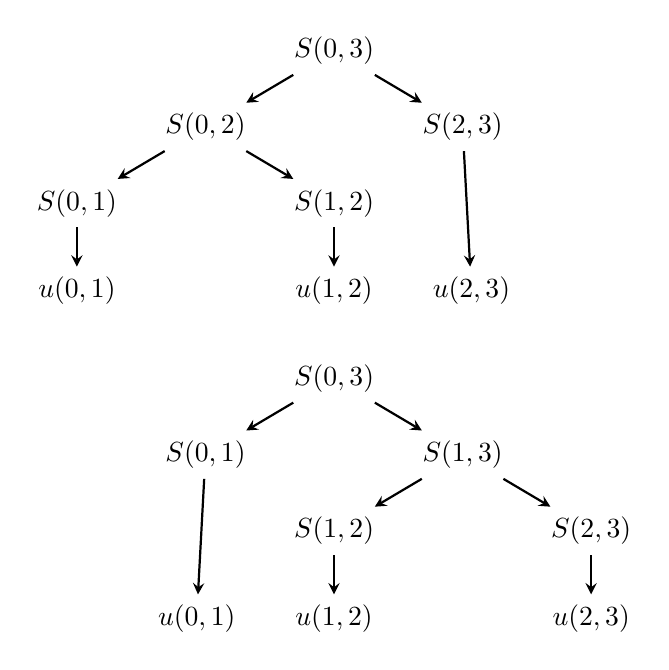
\begin{tikzpicture}[->,>=stealth,node distance = 0.5cm,thick]
\tikzstyle{v}=[]
\node[v]	(S03)	  					   		{$S(0,3)$};
\node[v]	(S02)  	[below left= of S03]		{$S(0,2)$};
\node[v]	(S23)  	[below right= of S03]		{$S(2,3)$};
\node[v]	(S01)  	[below left= of S02]		{$S(0,1)$};
\node[v]	(S12)  	[below right= of S02]		{$S(1,2)$};
\node[v]	(u01)  	[below = of S01]			{$u(0,1)$};
\node[v]	(u12)  	[below = of S12]			{$u(1,2)$};
\node[v]	(u23)  	[right = of u12]			{$u(2,3)$};
\node[v]	(T03)	[below = of u12]  			{$S(0,3)$};
\node[v]	(T01)  	[below left= of T03]		{$S(0,1)$};
\node[v]	(T13)  	[below right= of T03]		{$S(1,3)$};
\node[v]	(T12)  	[below left= of T13]		{$S(1,2)$};
\node[v]	(T23)  	[below right= of T13]		{$S(2,3)$};
\node[v]	(v12)  	[below = of T12]			{$u(1,2)$};
\node[v]	(v01)  	[left = of v12]				{$u(0,1)$};
\node[v]	(v23)  	[below = of T23]			{$u(2,3)$};
\path(S03)		edge	node			{}		(S02)
     (S03)		edge	node			{}		(S23)
     (S02)		edge	node			{}		(S01)
     (S02)		edge	node			{}		(S12)
     (S01)		edge	node			{}		(u01)
     (S12)		edge	node			{}		(u12)
     (S23)		edge	node			{}		(u23)
     (T03)		edge	node			{}		(T01)
     (T03)		edge	node			{}		(T13)
     (T13)		edge	node			{}		(T12)
     (T13)		edge	node			{}		(T23)
     (T01)		edge	node			{}		(v01)
     (T12)		edge	node			{}		(v12)
     (T23)		edge	node			{}		(v23);
\end{tikzpicture}
\caption{The two parse trees of "uuu" for the preceding grammar} \label{fig:M3}
\end{center}	
\end{figure}

Figure \ref{fig:M3} displays the two parse trees of the string "uuu" that is part of the above grammar. The meaning of the numbers at each node are as follows. Giving the string "uuu", number the string as shown:$$0 \quad u \quad 1 \quad u \quad 2 \quad u \quad 3$$ So $u(0,1)$ indicates that the $u$ of interest is between the numbers $0$ and $1$,  $u(1,2)$ indicates that the $u$ of interest is between the numbers $1$ and $2$, and so on. The numbers of the interior nodes are just natural extensions of this pattern.
\appendix
\section{Appendix Title}

This is the text of the appendix, if you need one.

\acks
We would like to thank Dr. Keshav Pingali for his guidance on this project. We would also like to thank Sepideh Maleki for helping us understand Scott's algorithm.

% We recommend abbrvnat bibliography style.

\bibliographystyle{abbrvnat}

% The bibliography should be embedded for final submission.

\begin{thebibliography}{}
\softraggedright

\bibitem[Bilardi and Pingali(2012)]{bilardi-pingali}
Gianfranco Bilardi, and Keshav Pingali. Parsing with Pictures. UTCS Tech Reports, 2012. This is a full TECHREPORT entry.

\bibitem[Scott(2008)]{scott}
Elizabeth Scott. SPPF-Style Parsing From Earley Recognisers. \textit{Electronic Notes in Theoretical Computer Science}, 203(53-67), 2008. This is a full ARTICLE entry.

\end{thebibliography}


\end{document}

%                       Revision History
%                       -------- -------
%  Date         Person  Ver.    Change
%  ----         ------  ----    ------

%  2013.06.29   TU      0.1--4  comments on permission/copyright notices

